% \begin{lstlisting}
% 底层实现原理

% 不同硬件上的针对性加速:
% 1. avx
% 2. arm
% 3. 鲲鹏
% 4. GPU
% \end{lstlisting}
In \MindQuantum, we use \Simulator to simulate quantum state. A \Simulator maintain a quantum state, as mentioned in section \ref{sec:sim_basic_usage}, methods start with `apply' will change this maintained quantum state, and methods start with `get' will not change anything but only extrude information from the quantum state.

Simulating quantum systems imposes high performance requirements on simulators. In \MindQuantum, we utilize C++ or CUDA as the underlying simulator implementation language, accelerating quantum simulations based on different hardware instruction sets. We adopt a policy-based development approach, optimizing the fundamental simulator interface for different instruction sets and encapsulating them into policy types. Building upon a unified quantum simulation framework, we generate different quantum simulators using various simulator policies, such as AVX-supported simulators, neon-supported simulators, and GPU-supported simulators.

\begin{figure}[ht]
    \centering
    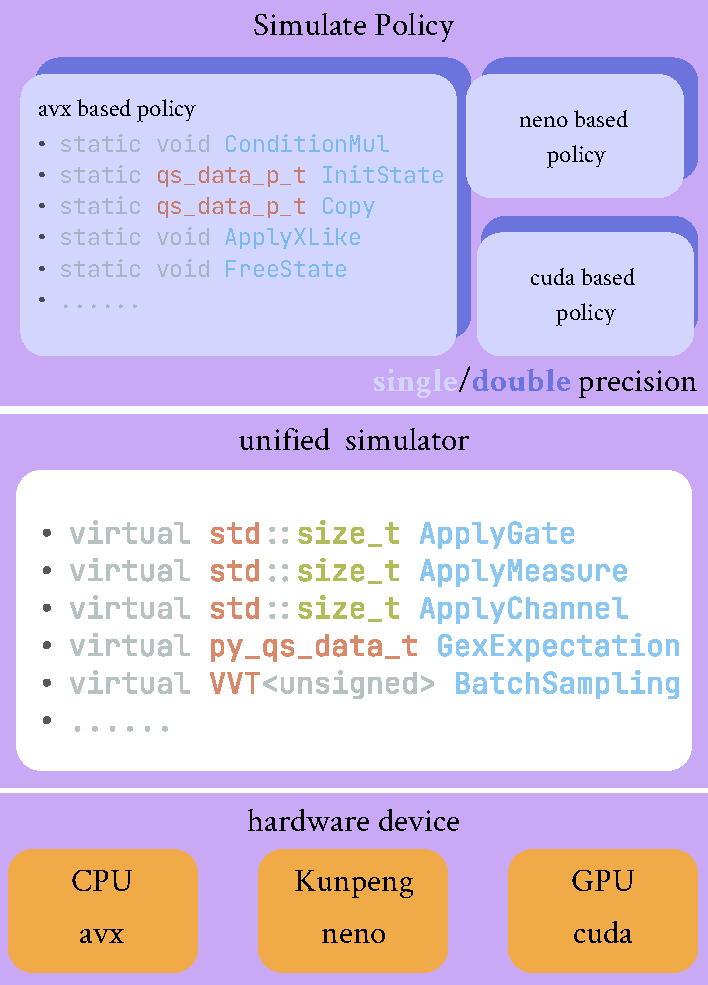
\includegraphics[scale=0.6]{./images/4_1_simulator_structure.pdf}
    \captionsetup{justification=raggedright,singlelinecheck=false}
    \caption{\label{4_1_sim_str} The layer structure of simulator in. The simulate policy layer applies quantum gate to quantum state based on actual simulation hardware. The unified simulator layer use different policy to finish circuit simulation and expectation and gradient calculation. The hardware device layer shows we support CPU, GPU and Kunpeng platform.}
\end{figure}

Depending on the specific quantum system being simulated, we have the option to choose between a full amplitude quantum simulator or a density matrix simulator. In \MindQuantum, these two simulators are referred to as `mqvector' and `mqmatrix', respectively. In the current \version version, the `mqvector' simulator also supports GPU acceleration and is named `mqvector\_gpu'. Both `mqvector' and `mqmatrix' use same design pattern in Fig.~\ref{4_1_sim_str}. Based on these simulators, noise simulation is also supported with the help of quantum channel, which will talked in section ~\ref{sec:noise_simulation}.
